\documentclass{beamer}

\usepackage{graphicx, subfigure}
\usepackage{amsmath}


% \usepackage{beamerthemesplit} // Activate for custom appearance


\title{\color{magenta}Introduction to Active Learning}

\author{ Nandana Sengupta}
\date{\color{olive}\today}

\begin{document}

\frame{\titlepage}

\frame{
\frametitle{\color{olive}Active Learning: Introduction}

\color{olive}
\begin{itemize}
\item<2-> ``n" objects: $\theta_1, \theta_2, \cdots \theta_n$.
\item<3-> ``m" individuals: $i_1, i_2, \cdots i_m$.
\item<4-> Aim is to get a ranking over the ``n" objects:
\begin{itemize}
\item<5->\color{magenta} global ranking: $\theta_2 \succ \theta_3  \succ \theta_1 \succ \theta_5 \succ \theta_6 \succ \theta_4$.
\item<6-> eg: web search queries, street safety queries.
\item<7->\color{magenta} matrix of individual rankings
\item<8-> eg: Netflix problem.
\end{itemize}
\item<9-> Issues in generating such rankings: \color{olive} costly queries, missing value problem, inefficiencies.
\item<10-> Typically random queries over ``n" objects $\Rightarrow$ number of queries: $n \choose 2$ 
\item<11-> \color{magenta}Inefficient! This is where Active Learning comes in.
\end{itemize}
}



\frame{
\frametitle{\color{olive}Active Learning: Introduction}

\color{olive}
\begin{itemize}
\item<2-> \color{magenta} ``Active Ranking using Pairwise Comparisons" -- Jamieson and Nowak (2011)
\item<3-> if there exists {\color{olive}$d<n$} features in $\mathcal{R}^d$ then can reduce order of queries: \color{olive} $\mathcal{O}(d \log n)$.
\item<4-> Main idea is to not query randomly but use these $d$ features.
\begin{itemize}
\item<5->\color{magenta} Reference Point in ``d"-dimensional space, say $r$.
\item<6-> Distance from $r$ determines ranking.
\item<7->\color{magenta} However $r$ is unknown -- so problem becomes estimating region where $r$ lies.
\item<8-> Some queries redundant -- example next.
\end{itemize}
\item<9-> \color{magenta} Assumptions
\begin{itemize}
\item<10-> {\color{olive}A1: Embedding} if $\theta_i \prec \theta_j$ then $\| \theta_i - r \| < \| \theta_j - r \|$.
\item<11-> {\color{olive}A2: Consistency} Every pairwise comparison is consistent with the global ranking.
\end{itemize}
\end{itemize}
}



\frame{
\frametitle{\color{olive}Active Learning: Example}
\centering
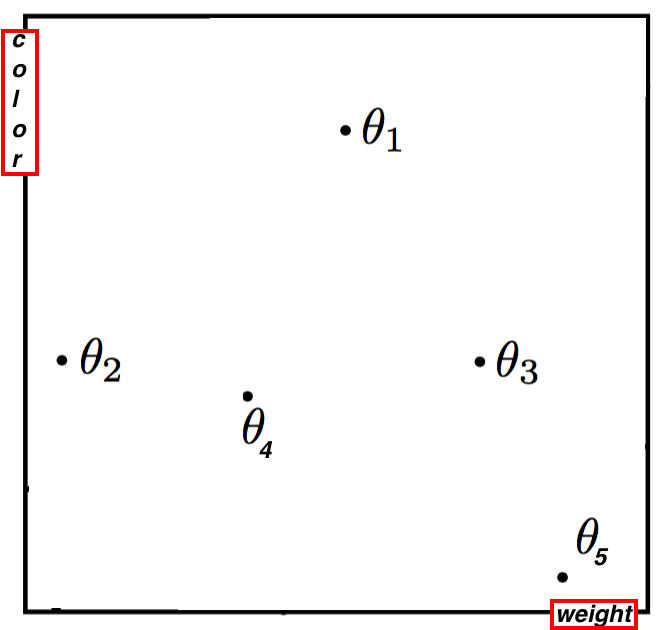
\includegraphics[width = 0.75\textwidth]{AL1}
}



\frame{
\frametitle{\color{olive}Active Learning: Example}
\centering
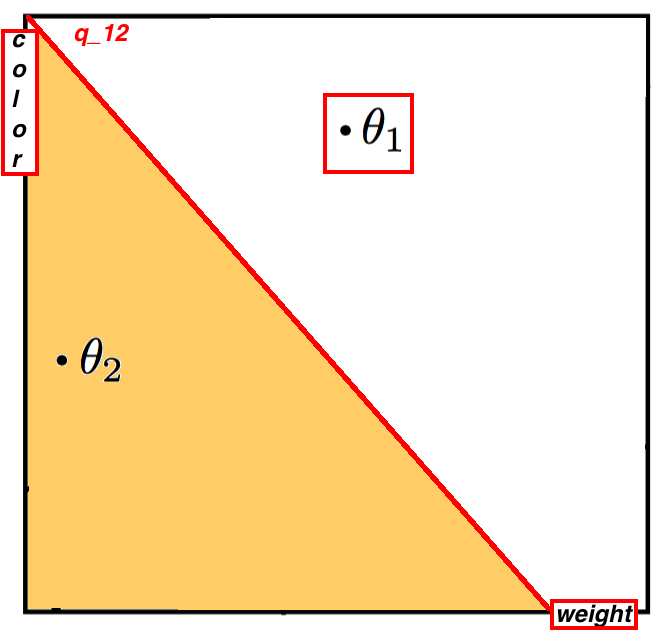
\includegraphics[width = 0.75\textwidth]{AL2}
}



\frame{
\frametitle{\color{olive}Active Learning: Example}
\centering
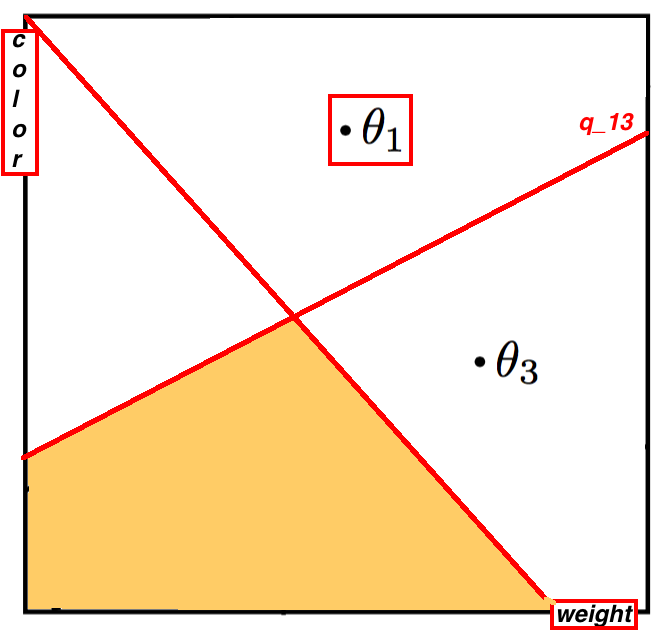
\includegraphics[width = 0.75\textwidth]{AL3}
}



\frame{
\frametitle{\color{olive}Active Learning: Example}
\centering
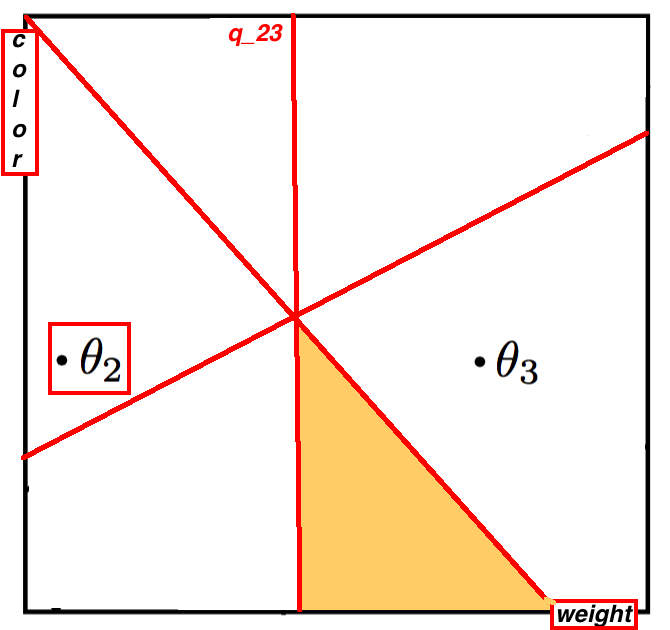
\includegraphics[width = 0.75\textwidth]{AL4}
}



\frame{
\frametitle{\color{olive}Active Learning: Example}
\centering
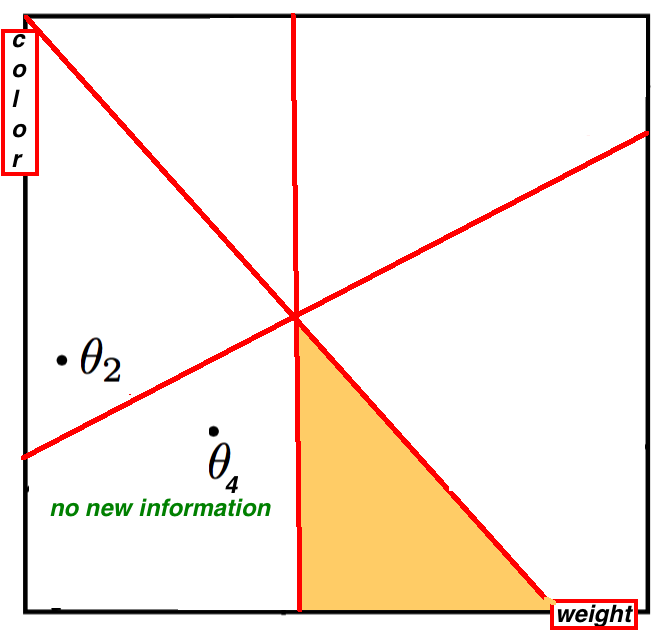
\includegraphics[width = 0.75\textwidth]{AL5}
}



\frame{
\frametitle{\color{olive}Active Learning: Example}
\centering
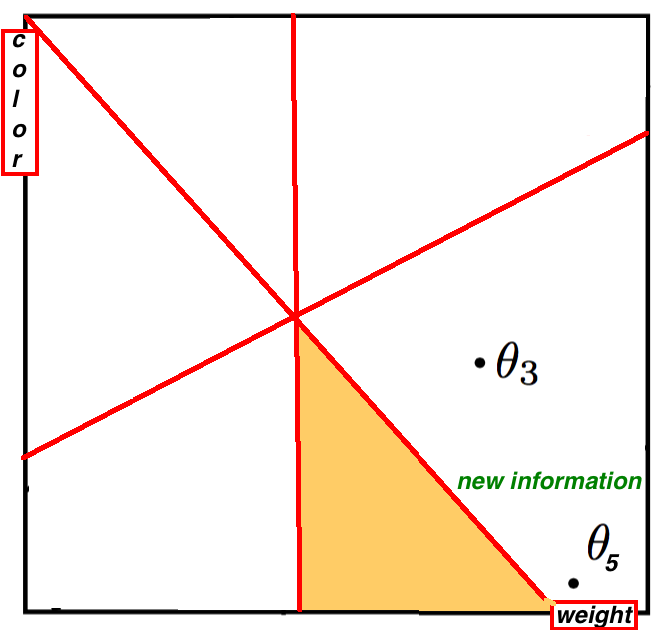
\includegraphics[width = 0.75\textwidth]{AL6}
}

\frame{
\frametitle{\color{olive}Active Learning: Possible Applications}
\begin{itemize}
\item<2-> Pairwise ranking surveys online.
\item<3-> \color{magenta}Eg: Street Score, All our ideas.
\item<4-> Generate global rankings by asking pairwise comparison queries.
\item<5-> Currently using random pairwise queries.
\item<6-> Opportunity for active learning algorithms. 
\end{itemize}
}


\frame{
\centering 

Thanks!
}


\end{document}

